\documentclass[11pt]{article}

\usepackage[margin=1in]{geometry}
\usepackage{setspace}
\onehalfspacing
\usepackage{graphicx}
\graphicspath{report_images/}
\usepackage{appendix}
\usepackage{listings}
\usepackage{float}
\usepackage{amsthm}
% The next three lines make the table and figure numbers also include section number
\usepackage{chngcntr}
\counterwithin{table}{section}
\counterwithin{figure}{section}
% Needed to make titling page without a page number
\usepackage{titling}

% DOCUMENT INFORMATION =================================================
\title {ECEN 429: Introduction to Digital Systems Design Laboratory \\ North Carolina Agricultural and Technical State University \\ Department of Electrical and Computer Engineering} % Declare Title
\author{Reporter: Chris Cannon\\ \and Partner: Nikiyah Beulah} % Declare authors
\date{February 8, 2018}
% ======================================================================

\begin{document}

\begin{titlingpage}
\maketitle
\begin{center}
	Lab 3
\end{center}
\end{titlingpage}

\section{Introduction}
This lab focuses on building increasingly complex systems that build on each other, which will give us more experience with integrating systems using components. Code reuse is important for any type of software development, including VHDL. Therefore, it is important that we understand how to nest components to build more complex systems from basic building blocks. We start by creating an adder circuit for two 2-bit numbers, and we build more complex circuits that utilize those systems for more advanced operations.

\section{Background, Design Solution, and Results}

\subsection{Problem 1 Bit Slicer}

\subsubsection{Background}
For this problem, we are to create a bit slicer that will add two 2-bit numbers 'a' and 'b', as well has handling a carry-in bit 'cin'.

\theoremstyle{definition}
\newtheorem{definition}{Definition}
\begin{definition}
Carry-in Bit: the carry-in bit represents a 1-bit overflow from a previous addition operation. Because a full adder is intended to be modular, and build adders of multiple bits, it is important that the previous operation be available. For purposes of this lab, the carry-in for a 1 bit adder will be tied to ground.
\end{definition}

The concept of a 2-bit adder was covered in Lab 2, so we had a good starting point for this lab. For reference, the truth table for a single 2-bit adder is defined in ~\ref{tab:fullAddTruthTable}.

\begin{table}[h]
\begin{center}
	\begin{tabular}{| l | l | l | l | l |}
		\hline
		A & B & CI & SUM & CO \\ \hline
		0 & 0 & 0 & 0 & 0 \\ \hline
		0 & 0 & 1 & 1 & 0 \\ \hline
		0 & 1 & 0 & 1 & 0 \\ \hline
		0 & 1 & 1 & 0 & 1 \\ \hline
		1 & 0 & 0 & 1 & 0 \\ \hline
		1 & 0 & 1 & 0 & 1 \\ \hline
		1 & 1 & 0 & 0 & 1 \\ \hline
		1 & 1 & 1 & 1 & 1 \\ \hline
	\end{tabular}
	\caption{\label{tab:fullAddTruthTable}Truth table for a full adder.}
	\label{tab:fullAddTruthTable}
\end{center}
\end{table}

\subsubsection{Design Solution}
To implement our design, we decided to use two full-adders. We were able to reuse our code from Lab 2 to create the full-adder entity, and then implement this design using two components. Because we abstracted our full-adder using a component, we had to write less actual code, which made our solution both cleaner and easier to read. For our inputs, we used 'a2' and 'a1' to represent our first 2-bit number, and 'b2' and 'b1' to represent our second 2-bit number. 'ci' of course represents out carry-in bit. The output sum is represented by bits `x2` and `x1`, and the carry-out bit is represented as `cout`. The truth table for this entire circuit is given in Table ~\ref{tab:stupidlyLongSlicerTruthTable}. The pin assignments for this design are given in Table ~\ref{tab:slicerPinAssignments}.

\begin{definition}
	Carry-out Bit: the carry-out bit represents a 1-bit overflow from the current addition operation. This can either be used to signal an error condition or to tie this adder in with multiple full adders. The result of this addition operation will either between 0 and 3. If the output is 2 or 3, the carry-out bit will be HIGH to signal that there is an additional bit needed to represent the results of this operation.
\end{definition}

\begin{table}[H]
\begin{center}
	\begin{tabular}{| l | l | l | l | l | l | l | l |}
		\hline
		cin & a2 & a1 & b2 & b1 & cout & x2 & x1 \\ \hline
		0 & 0 & 0 & 0 & 0 & 0 & 0 & 0 \\ \hline
		0 & 0 & 0 & 0 & 1 & 0 & 0 & 1 \\ \hline
		0 & 0 & 0 & 1 & 0 & 0 & 1 & 0 \\ \hline
		0 & 0 & 0 & 1 & 1 & 0 & 1 & 1 \\ \hline
		0 & 0 & 1 & 0 & 0 & 0 & 0 & 1 \\ \hline
		0 & 0 & 1 & 0 & 1 & 0 & 1 & 0 \\ \hline
		0 & 0 & 1 & 1 & 0 & 0 & 1 & 1 \\ \hline
		0 & 0 & 1 & 1 & 1 & 1 & 0 & 0 \\ \hline
		0 & 1 & 0 & 0 & 0 & 0 & 1 & 0 \\ \hline
		0 & 1 & 0 & 0 & 1 & 0 & 1 & 1 \\ \hline
		0 & 1 & 0 & 1 & 0 & 1 & 0 & 0 \\ \hline
		0 & 1 & 0 & 1 & 1 & 1 & 0 & 1 \\ \hline
		0 & 1 & 1 & 0 & 0 & 0 & 1 & 1 \\ \hline
		0 & 1 & 1 & 0 & 1 & 1 & 0 & 0 \\ \hline
		0 & 1 & 1 & 1 & 0 & 1 & 0 & 1 \\ \hline
		0 & 1 & 1 & 1 & 1 & 1 & 1 & 0 \\ \hline
		1 & 0 & 0 & 0 & 0 & 0 & 0 & 1 \\ \hline
		1 & 0 & 0 & 0 & 1 & 0 & 1 & 0 \\ \hline
		1 & 0 & 0 & 1 & 0 & 0 & 1 & 1 \\ \hline
		1 & 0 & 0 & 1 & 1 & 1 & 0 & 0 \\ \hline
		1 & 0 & 1 & 0 & 0 & 0 & 1 & 0 \\ \hline
		1 & 0 & 1 & 0 & 1 & 0 & 1 & 1 \\ \hline
		1 & 0 & 1 & 1 & 0 & 1 & 0 & 0 \\ \hline
		1 & 0 & 1 & 1 & 1 & 1 & 0 & 1 \\ \hline
		1 & 1 & 0 & 0 & 0 & 0 & 1 & 1 \\ \hline
		1 & 1 & 0 & 0 & 1 & 1 & 0 & 0 \\ \hline
		1 & 1 & 0 & 1 & 0 & 1 & 0 & 1 \\ \hline
		1 & 1 & 0 & 1 & 1 & 1 & 1 & 0 \\ \hline
		1 & 1 & 1 & 0 & 0 & 1 & 0 & 0 \\ \hline
		1 & 1 & 1 & 0 & 1 & 1 & 0 & 1 \\ \hline
		1 & 1 & 1 & 1 & 0 & 1 & 1 & 0 \\ \hline
		1 & 1 & 1 & 1 & 1 & 1 & 1 & 1 \\ \hline
	\end{tabular}
	\caption{\label{tab:stupidlyLongSlicerTruthTable}Truth table for the problem 1 solution.}
\end{center}
\end{table}

\begin{table}[H]
\begin{center}
	\begin{tabular}{| l | l | l |}
		\hline
		Bit & Label & Port \\ \hline
		a1 & Switch 0 & V17 \\ \hline
		a2 & Switch 1 & V16 \\ \hline
		b1 & Switch 2 & W16 \\ \hline
		b2 & Switch 3 & W17 \\ \hline
		cin & Switch 4 & W15 \\ \hline
		x1 & LED 0 & U16 \\ \hline
		x2 & LED 1 & E19 \\ \hline
		cout & LED 2 & V19 \\ \hline
	\end{tabular}
	\caption{\label{tab:slicerPinAssignments}Port assignment for each bit used in Problem 1.}
\end{center}
\end{table}

\subsubsection{Results}

%TODO: ADD PHOTOS HERE

\subsection{Problem 2 2:1 Multiplexer}

\subsubsection{Background}
Using the bit slicer developed in Problem 1, we will feed the outputs into a 2:1 multiplexer with a 1-bit `sel` input. 

\begin{definition}
	Multiplexer: A multiplexer, or mux, is a digital device that can "pass-through" values depending on a selector input. For example, a 2:1 mux with a 1-bit selector and inputs 'a' and 'b' will output input 'a' when the selector input is '0' or LOW and will output 'b' when the selector input is '1' or HIGH.
\end{definition}

The multiplexer in this problem is supposed to output the sum of the bit slicer operation when the 'sel' bit is '1' or HIGH. The sum refers to \textit{only} the two bit output of the sum operation. In this lab, we referred to these outputs as 'x2' and 'x1', where 'x2' is the most significant bit. When the 'sel' bit is '0' or LOW, the circuit is supposed to output the carry-out bit 'cout'. 

\subsubsection{Design Solution}
To implement this design, we reused the code from Problem one, and used it as a component. Therefore, we only had to declare and instantiate the component, not redefine the architecture. Based on the assignment given in the Background section above, we knew that we had to basically double our truth table. If the 'sel' bit is HIGH or '1', we will output 'x2' and 'x1'. When the 'sel' bit is LOW or '0', we will output just the 'cout' bit. Tables ~\ref{tab:selOneTruthTable} and ~\ref{tab:selZeroTruthTable} provide the truth tables for this design. We have summarized our port assignments in Table ~\ref{tab:ledMuxPorts}.

\begin{table}[H]
\begin{center}
	\begin{tabular}{| l | l | l |}
		\hline
		Bit & Label & Port \\ \hline
		a1 & Switch 0 & V17 \\ \hline
		a2 & Switch 1 & V16 \\ \hline
		b1 & Switch 2 & W16 \\ \hline
		b2 & Switch 3 & W17 \\ \hline
		cin & Switch 4 & W15 \\ \hline
		sel & Switch 5 & V15 \\ \hline
		x1 & LED 0 & U16 \\ \hline
		x2 & LED 1 & E19 \\ \hline
		cout & LED 2 & V19 \\ \hline
	\end{tabular}
	\caption{\label{tab:ledMuxPorts}Input and output pin assignments for the multiplexer circuit.}
\end{center}	
\end{table}


\begin{table}[H]
\begin{center}
	\begin{tabular}{| l | l | l | l | l | l | l | l | l |}
		\hline
		sel & cin & a2 & a1 & b2 & b1 & cout & x2 & x1 \\ \hline
		1 & 0 & 0 & 0 & 0 & 0 & 0 & 0 & 0 \\ \hline
		1 & 0 & 0 & 0 & 0 & 1 & 0 & 0 & 1 \\ \hline
		1 & 0 & 0 & 0 & 1 & 0 & 0 & 1 & 0 \\ \hline
		1 & 0 & 0 & 0 & 1 & 1 & 0 & 1 & 1 \\ \hline
		1 & 0 & 0 & 1 & 0 & 0 & 0 & 0 & 1 \\ \hline
		1 & 0 & 0 & 1 & 0 & 1 & 0 & 1 & 0 \\ \hline
		1 & 0 & 0 & 1 & 1 & 0 & 0 & 1 & 1 \\ \hline
		1 & 0 & 0 & 1 & 1 & 1 & 0 & 0 & 0 \\ \hline
		1 & 0 & 1 & 0 & 0 & 0 & 0 & 1 & 0 \\ \hline
		1 & 0 & 1 & 0 & 0 & 1 & 0 & 1 & 1 \\ \hline
		1 & 0 & 1 & 0 & 1 & 0 & 0 & 0 & 0 \\ \hline
		1 & 0 & 1 & 0 & 1 & 1 & 0 & 0 & 1 \\ \hline
		1 & 0 & 1 & 1 & 0 & 0 & 0 & 1 & 1 \\ \hline
		1 & 0 & 1 & 1 & 0 & 1 & 0 & 0 & 0 \\ \hline
		1 & 0 & 1 & 1 & 1 & 0 & 0 & 0 & 1 \\ \hline
		1 & 0 & 1 & 1 & 1 & 1 & 0 & 1 & 0 \\ \hline
		1 & 1 & 0 & 0 & 0 & 0 & 0 & 0 & 1 \\ \hline
		1 & 1 & 0 & 0 & 0 & 1 & 0 & 1 & 0 \\ \hline
		1 & 1 & 0 & 0 & 1 & 0 & 0 & 1 & 1 \\ \hline
		1 & 1 & 0 & 0 & 1 & 1 & 0 & 0 & 0 \\ \hline
		1 & 1 & 0 & 1 & 0 & 0 & 0 & 1 & 0 \\ \hline
		1 & 1 & 0 & 1 & 0 & 1 & 0 & 1 & 1 \\ \hline
		1 & 1 & 0 & 1 & 1 & 0 & 0 & 0 & 0 \\ \hline
		1 & 1 & 0 & 1 & 1 & 1 & 0 & 0 & 1 \\ \hline
		1 & 1 & 1 & 0 & 0 & 0 & 0 & 1 & 1 \\ \hline
		1 & 1 & 1 & 0 & 0 & 1 & 0 & 0 & 0 \\ \hline
		1 & 1 & 1 & 0 & 1 & 0 & 0 & 0 & 1 \\ \hline
		1 & 1 & 1 & 0 & 1 & 1 & 0 & 1 & 0 \\ \hline
		1 & 1 & 1 & 1 & 0 & 0 & 0 & 0 & 0 \\ \hline
		1 & 1 & 1 & 1 & 0 & 1 & 0 & 0 & 1 \\ \hline
		1 & 1 & 1 & 1 & 1 & 0 & 0 & 1 & 0 \\ \hline
		1 & 1 & 1 & 1 & 1 & 1 & 0 & 1 & 1 \\ \hline
	\end{tabular}
	\caption{\label{tab:selOneTruthTable}This table shows the outputs displayed when the 'sel' bit is '1' or HIGH. The only output should be from the sum bits 'x2' and 'x1'.}
\end{center}	
\end{table}

\begin{table}[H]
\begin{center}
	\begin{tabular}{| l | l | l | l | l | l | l | l | l |}
		\hline
		sel & cin & a2 & a1 & b2 & b1 & cout & x2 & x1 \\ \hline
		0 & 0 & 0 & 0 & 0 & 0 & 0 & 0 & 0 \\ \hline
		0 & 0 & 0 & 0 & 0 & 1 & 0 & 0 & 0 \\ \hline
		0 & 0 & 0 & 0 & 1 & 0 & 0 & 0 & 0 \\ \hline
		0 & 0 & 0 & 0 & 1 & 1 & 0 & 0 & 0 \\ \hline
		0 & 0 & 0 & 1 & 0 & 0 & 0 & 0 & 0 \\ \hline
		0 & 0 & 0 & 1 & 0 & 1 & 0 & 0 & 0 \\ \hline
		0 & 0 & 0 & 1 & 1 & 0 & 0 & 0 & 0 \\ \hline
		0 & 0 & 0 & 1 & 1 & 1 & 1 & 0 & 0 \\ \hline
		0 & 0 & 1 & 0 & 0 & 0 & 0 & 0 & 0 \\ \hline
		0 & 0 & 1 & 0 & 0 & 1 & 0 & 0 & 0 \\ \hline
		0 & 0 & 1 & 0 & 1 & 0 & 1 & 0 & 0 \\ \hline
		0 & 0 & 1 & 0 & 1 & 1 & 1 & 0 & 0 \\ \hline
		0 & 0 & 1 & 1 & 0 & 0 & 0 & 0 & 0 \\ \hline
		0 & 0 & 1 & 1 & 0 & 1 & 1 & 0 & 0 \\ \hline
		0 & 0 & 1 & 1 & 1 & 0 & 1 & 0 & 0 \\ \hline
		0 & 0 & 1 & 1 & 1 & 1 & 1 & 0 & 0 \\ \hline
		0 & 1 & 0 & 0 & 0 & 0 & 0 & 0 & 0 \\ \hline
		0 & 1 & 0 & 0 & 0 & 1 & 0 & 0 & 0 \\ \hline
		0 & 1 & 0 & 0 & 1 & 0 & 0 & 0 & 0 \\ \hline
		0 & 1 & 0 & 0 & 1 & 1 & 1 & 0 & 0 \\ \hline
		0 & 1 & 0 & 1 & 0 & 0 & 0 & 0 & 0 \\ \hline
		0 & 1 & 0 & 1 & 0 & 1 & 0 & 0 & 0 \\ \hline
		0 & 1 & 0 & 1 & 1 & 0 & 1 & 0 & 0 \\ \hline
		0 & 1 & 0 & 1 & 1 & 1 & 1 & 0 & 0 \\ \hline
		0 & 1 & 1 & 0 & 0 & 0 & 0 & 0 & 0 \\ \hline
		0 & 1 & 1 & 0 & 0 & 1 & 1 & 0 & 0 \\ \hline
		0 & 1 & 1 & 0 & 1 & 0 & 1 & 0 & 0 \\ \hline
		0 & 1 & 1 & 0 & 1 & 1 & 1 & 0 & 0 \\ \hline
		0 & 1 & 1 & 1 & 0 & 0 & 1 & 0 & 0 \\ \hline
		0 & 1 & 1 & 1 & 0 & 1 & 1 & 0 & 0 \\ \hline
		0 & 1 & 1 & 1 & 1 & 0 & 1 & 0 & 0 \\ \hline
		0 & 1 & 1 & 1 & 1 & 1 & 1 & 0 & 0 \\ \hline
	\end{tabular}
	\caption{\label{tab:selZeroTruthTable}This table shows the outputs displayed when the 'sel' bit is '0' or LOW. The only output should be the carry-out bit 'cout'.}
\end{center}
\end{table}

\subsubsection{Results}

% ADD PHOTOS HERE

\subsection{Problem 3 2:1 Multiplexer with Seven-Segment Output}

\subsubsection{Background}
For this problem, we are to utilize the seven-segment display to output our result from the circuit in Problem 2. Basically, if we are to output the sum, then we should display 0, 1, 2, or 3 on the seven-segment display. If we are to display the carry-out, then we will display 0 or 1.

\subsubsection{Design Solution}
The truth table for this circuit will be the same truth table shown in Figures ~\ref{tab:selZeroTruthTable} and ~\ref{tab:selOneTruthTable}, however output will be shown utilizing the seven-segment displays. A diagram of a segment display is shown in Figure ~\ref{fig:sevenSegFigure}.

\begin{figure}[h]
\begin{center}
	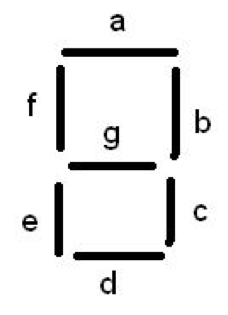
\includegraphics[width=0.2\textwidth]{../Lab2/report-images/img1.png}
	\caption{\label{fig:sevenSegFigure}Diagram of seven-segment display showing the assigned letter for each segment.}
\end{center}
\end{figure}

\end{document}
